\documentclass{report}
\usepackage[margin=1in]{geometry}
\usepackage{setspace}
\usepackage{times}
\title{
	\textsc{ \small
		Washington State University \\
		School of Electrical Engineering and Computer Science \\
		EE 352, Electrical Engineering Laboratory
	} \\
	{\textsc{\small Lab \#7}} \\
	MOSFET circuits
}

\author{
	Name: Kevin Evans \\
	Partner: Jacob Hnatiak, Aman Amad al-Ameedi
}
\date{Due Date: March 10, 2020}

% start sections at 1 with subsections to 1.1, 1.2...
\renewcommand{\thesection}{\arabic{section}}

%alias for vpp/rms
\newcommand{\pp}{_{pp}}
\newcommand{\rms}{_{rms}}
\newcommand{\Vpp}{\V\pp}
\newcommand{\Vrms}{\V\rms}

\usepackage{siunitx}
\usepackage{threeparttable}
\usepackage{booktabs}
\usepackage{multirow}
\usepackage{graphicx}
\usepackage{float}
\usepackage{amssymb,amsmath}
\usepackage{physics,cancel}
\usepackage{listings}
\usepackage{steinmetz} % \phase{}
\usepackage{mathtools} % for '\mathclap' macro
\usepackage{caption,subcaption} %multiline captions; subfigures


\begin{document}
\maketitle

\section*{Lab Overview}
% what was the lab about and the outcome?
In this lab, we experimentally determined the characteristics of metal-oxide-semiconductor field-effect transistors (MOSFETs) for two types of transistors: the NMOS and PMOS. Throughout the lab, we saw various applications of MOSFETs, including a voltage-controlled resistor and a buffer amplifier. These applications use the unique characteristics and operating regions of MOSFETs.


%%%%%%%%%%%%%%%%%%%%%%%%%%%%%%%%%%%%%%%%%%%%%%%%%%%%%%%%%%%%%
\section{MOSFET I-V characteristics}

\subsection{Purpose}
% purpose of the experiment and its specs and/or design requirements
In this experiment, we used the Tek 571 curve tracer and found the current-voltage (I-V) curves for the ZVN2110A (NMOS) and ZVP2110A (PMOS) transistor. From these curves, we determined the threshold voltage and other attributes of each transistor.

\subsection{Theoretical background}
% background and its theory of operation, circuit diagrams, the main equations, results from the prelab
In this experiment, we will use both NMOS and PMOS transistors. Each of these transistors require a minimum threshold voltage $V_t$ across the gate to operate. Below this voltage, current is virtually unable to flow across the transistor as the channel is not established. Above this, we can vary the drain-source voltage relative to the gate-source voltage. Changing these parameters will affect how the current flows, depending on whether the transistor is operating in the triode or saturation region. These regions and their respective currents are shown in Table \ref{table:exp1current} below.

\bgroup
\def\arraystretch{2}%  1 is the default, change whatever you need
\begin{table}[H]
	\centering
	\caption{Equations for currents through the drain terminal for both the NMOS and PMOS transistors.}
	\label{table:exp1current}
	\begin{tabular}{ccccl}
		\specialrule{1.2pt}{0pt}{-3pt}
		Transistor Type & \multicolumn{2}{c}{Conditions} & Region & \multicolumn{1}{c}{Current} \\
		\hline
		\multirow{3}{*}{NMOS} & $V_{GS} < V_t$ & & Cutoff & $I_D = 0$ \\
			\cline{2-5}
			& \multirow{2}{*}{$V_{GS}\ge V_t$} & $V_{DS} < V_{OV}$ & Triode & $I_D = k_n \left[ \left(V_{GS} - V_t\right)V_{DS} - \dfrac{1}{2} \left(V_{DS}\right)^2\right]$ \\
			\cline{3-5}
			& & $V_{DS} \ge V_{OV}$ & Saturation & $I_D = \dfrac{k_n}{2} \left(V_{GS} - V_t\right)^2 \left(1 + \lambda V_{DS}\right)$  \\
		\hline
		\multirow{3}{*}{PMOS} & $V_{SG} < \abs{V_t}$ & & Cutoff & $I_D = 0$ \\
		\cline{2-5}
		& \multirow{2}{*}{$V_{SG} \ge \abs{V_t}$} & $V_{SD} < \abs{V_{OV}}$ & Triode & $I_D = k_n \left[ \left(V_{SG} - \abs{V_t}\right)V_{SD} - \dfrac{1}{2} \left(V_{SD}\right)^2\right]$ \\
		\cline{3-5}
		& & $V_{SD} \ge \abs{V_{OV}}$ & Saturation & $I_D = \dfrac{k_n}{2} \left(V_{SG} - V_t\right)^2 \left(1 + \lambda V_{SD}\right)$  \\
		\bottomrule
	\end{tabular}
\end{table}

\egroup
\noindent In the saturation region, the transconductance $g_m$ is defined as \begin{equation*}
	g_m = \eval{ \pdv{i_D}{v_{GS}} }_{I_D} \approx \frac{\Delta I_D}{\Delta V_{GS}}
\end{equation*}
We can use the equations from Table \ref{table:exp1current} and evaluate the derivative to find the transconductance as \begin{align}
	g_m & = \pdv{V_{GS}} \left[\frac{k_n}{2} \left(V_{GS} - V_t\right)^2 \left(1 + \lambda V_{DS}\right)\right]\notag \\
		& = k_n \left(V_{GS} - V_t\right)\left(1 + \lambda V_{DS}\right) \label{eq:exp1g}
\end{align}
Additionally, the transconductance can be estimated as \begin{align}
	g_m & = \sqrt{2 K_n I_D}  \approx \frac{2I_D}{V_{GS} - V_t}
\end{align}
From the datasheet of the ZVN2110A and ZVP2110A, the threshold voltages were in the range of \begin{align*}
	V_t & = 0.8 \text{ to } \SI{2.4}{\V} \text{ at } \SI{1}{\mA} && \text{ZVN2110A} \\
	V_t & = -1.5 \text{ to } \SI{-3.5}{\V} \text{ at } \SI{-1}{\mA} && \text{ZVP2110A}
\end{align*}
\subsection{Procedure}
The follow steps were carried out, as instructed by the lab assignment.

\subsubsection{A. Obtain the current-voltage curve for the NMOS transistor.}
\begin{enumerate}
	\item Using the Tek 571 curve tracer, the $I_D$-$V_{GS}$ curve was obtained for the ZVN2110A NMOS transistor. From this plot, the experimental threshold voltage can be obtained.
	\item The transistor was attached to the curve tracer with both the drain/gate terminals shorted in the drain socket.
	\item The curve parameters were set to:
	
	\begin{tabular}{ll}
		Function: & Acquisition \\
		Type: & NFET \\
		$V_{DS}$ max: & \SI{5}{\V} \\
		$I_S$ max: & \SI{10}{\mA} \\
		$V_g$/step: & \SI{0.2}{\V} \\
		Offset: & \SI{0}{\V} \\
		Steps: & 1 \\
		$R_\mathrm{load}$: & \SI{0.25}{\ohm} \\
		$P$ max: & \SI{0.5}{\W}
	\end{tabular}

	Then, the acquisition was started.
	\item A diode curve plot was obtained and the threshold voltage $V_t$ was found using a cursor on the plot. A photo was obtained of the screen as well.
\end{enumerate}
\subsubsection{B. Obtain current-voltage curves at multiple steps for the NMOS.}
\begin{enumerate}
	\item The NMOS transistor was connected in the normal configuration on the socket on the curve tracer.
	\item The curve tracer was configured to step through several gate-source voltages.
	\item The curve tracer parameters were set to:
	
	\begin{tabular}{ll}
	Function: & Acquisition \\
	Type: & NFET \\
	$V_{DS}$ max: & \SI{10}{\V} \\
	$I_S$ max: & \SI{50}{\mA} \\
	$V_g$/step: & \SI{0.1}{\V} \\
	Offset: & $V_t  + \SI{0.1}{\V}$ \\
	Steps: & 5 \\
	$R_\mathrm{load}$: & \SI{0.25}{\ohm} \\
	$P$ max: & \SI{0.5}{\W}
	\end{tabular}
	
	And the acquisition was started.
	\item Six curves were obtained for several values of $V_{GS}$.
	\item Several photos were taken of these curves.
\end{enumerate}

\subsubsection{C. Obtain the current-voltage curve for the PMOS transistor.}
Step A(1--4) was repeated for the PMOS transistor.
\subsubsection{D. Obtain current-voltage curves at multiple steps for the PMOS.}
Step B(1--5) was repeated for the PMOS transistor.

\subsubsection{E. Estimating transistor parameters from obtained graphs}
\begin{enumerate}
	\item The pictures of the curve tracer screens were transferred onto a computer, so that the transconductance and threshold voltages could be estimated.
	\item The threshold voltages were measured from the pictures, as well as the cursor feature.
	\item The transconductance $g_m$ was estimated using the slope of $I_D$-$V_{GS}$ curve for the NMOS transistor. From this $g_m$ value, the parameter $k_n$ was estimated.
	\item Step 3 was repeated for the PMOS transistor.
	\item The channel modulation index $\lambda$ was estimated for each transistor.
	\item On the NMOS $I$-$V_{DS}$ family of curves, six different points were chosen with three points in the saturation and three in the triode region. These points were recorded and used to calculate an average value of $k_n$.
	\item Step 6 was repeated for the PMOS transistor.
\end{enumerate}

\subsubsection{Post lab: OrCAD PSPICE simulation}
Using the parameters estimated, the $i_D$-$v_{DS}$ curves were obtained for both the n- and p-channel MOSFETs. These were compared to the experimental curves. The results of the simulation are shown in the appendix, closely matching the $I$-$V$ curves near the threshold voltage, later departing the measured curves as the gate voltage increases.
\subsection{Results and analysis}
% state all measured values, graphs, tables, and figs.
% state any deviation from theoretical expected values
% use tables and graphs
% * must justify error in results otherwise the experiment failed
For both transistors, the threshold voltage was captured using the on-screen cursors. From the curves, a transconductance were obtained using the slope at an arbitrary point in the forward-biased ``on'' region, as shown in Figure \ref{fig:diodes}. The process transconductance $k$ was found using equation \eqref{eq:exp1g}. These values are noted below in Table \ref{table:exp1values}.

From the $I$-$V_{DS}$ family of curves, six points were taken for both the NMOS and PMOS transistors, from both the triode and saturation region. These screens are shown in Figure \ref{fig:families}. From this, the process transconductance values $k$ were calculated for each by taking points from both regions and using their respective equation from Table \ref{table:exp1current} and solving for $k$. These values are shown in Table \ref{table:exp1family}. There is some variation between the $k$ values and the error could be due to the inaccuracies when measuring using the curve tracer, as the rounded screen could lead to some imprecise measurements when eyeballing it.

\begin{figure}[H]
	\centering
	\begin{subfigure}{0.45\textwidth}
		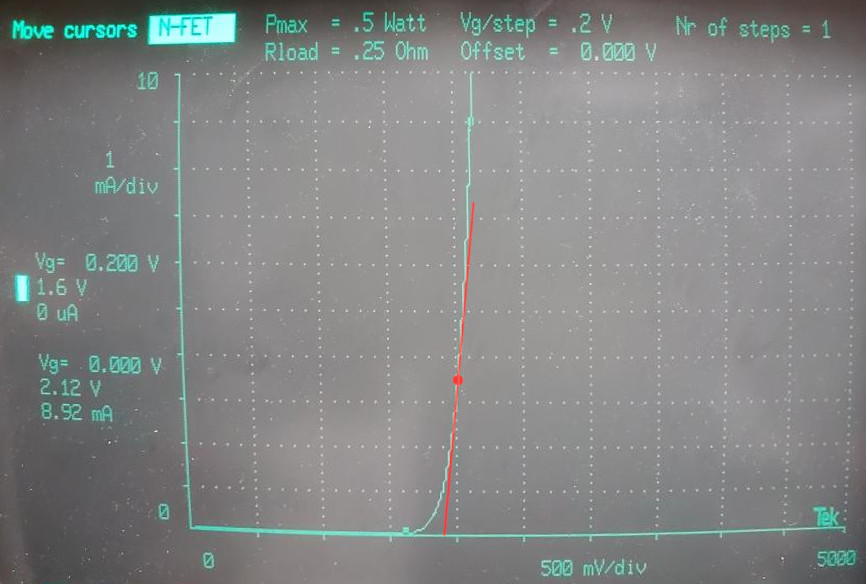
\includegraphics[width=\linewidth]{screennfet}
		\caption{NMOS I-V characteristics.}
		\label{fig:screennfet}
	\end{subfigure}
	\hfill
	\begin{subfigure}{0.45\textwidth}
		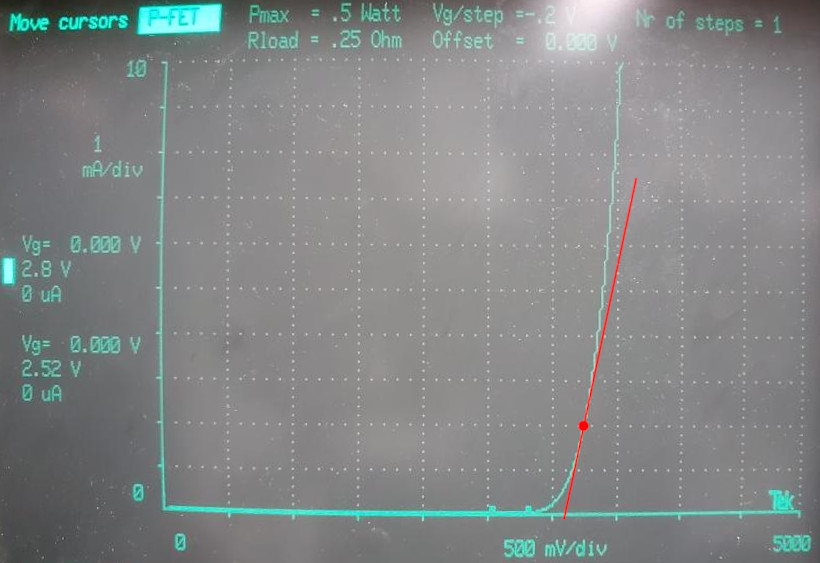
\includegraphics[width=\linewidth]{screenpfet}
		\caption{PMOS I-V characteristics.}
		\label{fig:screenpfet}
	\end{subfigure}
	\caption{The I-V characteristics for each transistor in the diode configuration.}
	\label{fig:diodes}
\end{figure}

\begin{figure}[H]
	\centering
	\begin{subfigure}{0.45\textwidth}
		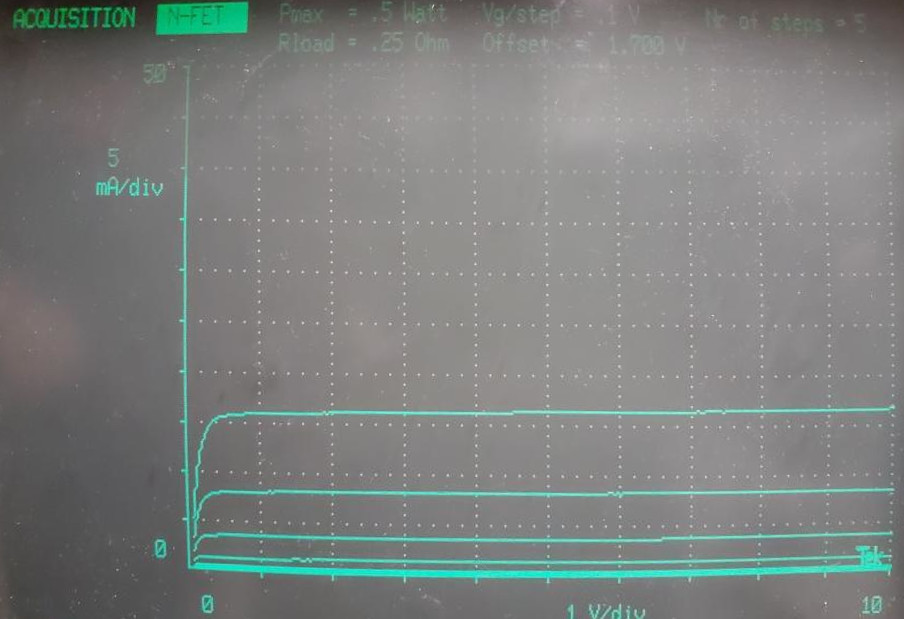
\includegraphics[width=\linewidth]{familynfet}
		\caption{NMOS I-V characteristics.}
	\end{subfigure}
	\hfill
	\begin{subfigure}{0.45\textwidth}
		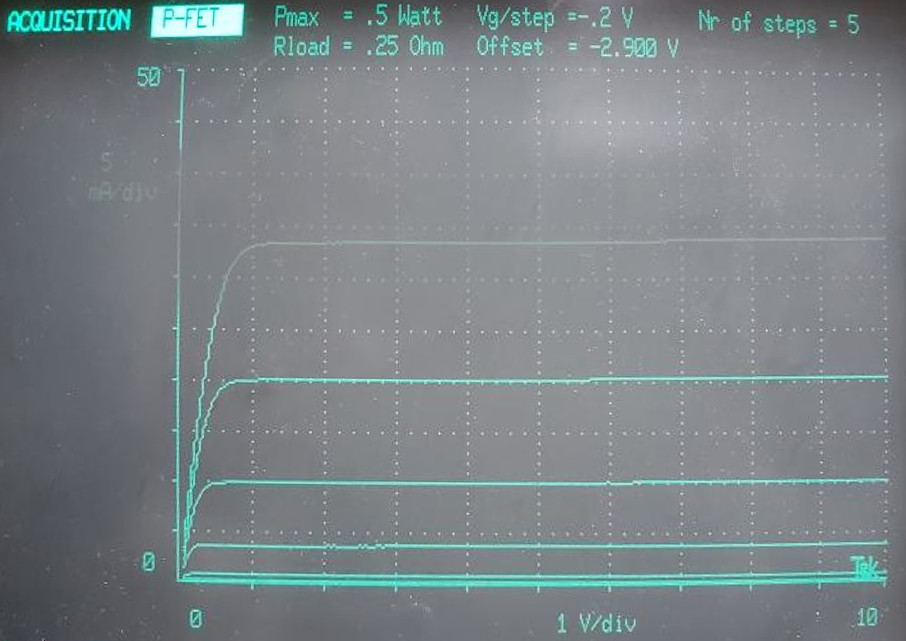
\includegraphics[width=\linewidth]{familypfet}
		\caption{PMOS I-V characteristics.}
	\end{subfigure}
	\caption{The I-Vds family of curves for both transistors.}
	\label{fig:families}
\end{figure}

\begin{table}[H]
	\centering
	\caption{Experimental threshold and transconductance values of the NMOS and PMOS transistors in Experiment 1.}
	\label{table:exp1values}
	\begin{threeparttable}
		\begin{tabular}{lcccc}
			\toprule
			\multirow{2}{*}{} & \multirow{2}{*}{Symbol} & \multicolumn{2}{c}{\footnotesize Transistor} & \multirow{2}{*}{Unit} \\
			& & NMOS & PMOS & \\
			\midrule
			Threshold voltage & $V_{t}$ & $1.60$ & $2.80$ & \si{\V}\\
			Transconductance & $g_m$ & $0.0278$ & $0.01364$ & \si{\per\ohm} \\
			Process transconductance & $k$ & $0.1104$ & $0.0465$ & \si{\A\per\V\squared} \\
			Channel modulation index & $\lambda$ & $0.00523$ & $0.001472$ & \si{\per\V} \\
			\bottomrule
		\end{tabular}
	\end{threeparttable}
\end{table}

\begin{table}[H]
	\centering
	\caption{Experimental $k$ values calculated using the family of curves in both the triode and saturation regions.}
	\label{table:exp1family}
	\begin{threeparttable}
		\begin{tabular}{cccccc}
			\toprule
			& $I_D$ & $V_{GS}$ & $V_{DS}$ & $k$ & \multirow{2}{*}{Region} \\
			& {\footnotesize \si{[\mA]}} & {\footnotesize \si{[\V]}}
				& {\footnotesize \si{[\mV]}}
				& {\footnotesize \si{[\A\per\V\squared]}}
				& \\
			\midrule
			\multirow{6}{*}{NMOS} & $2.0$ & $2.1$ & $50$ & $0.084$ & \multirow{3}{*}{Triode} \\
			& $5.7$ & $2.2$ & $100$ & $0.104$ & \\
			& $9.0$ & $2.3$ & $100$ & $0.138$ & \\
			\cline{2-6}
			& $4.2$ & $2.1$ & $10000$ & $0.032$ & \multirow{3}{*}{Saturation} \\
			& $9.0$ & $2.2$ & $10000$ & $0.048$ & \\
			& $17.60$ & $2.3$ & $10000$ & $0.068$ & \\
			\midrule
			\multirow{6}{*}{PMOS} & $7.5$ & $-3.5$ & $200$ & $0.063$ & \multirow{3}{*}{Triode} \\
& $11$ & $-3.7$ & $200$ & $0.069$ & \\
& $13$ & $-3.9$ & $200$ & $0.065$ & \\
			\cline{2-6}
& $10$ & $-3.5$ & $1400$ & $0.040$ & \multirow{3}{*}{Saturation} \\
& $20$ & $-3.7$ & $1400$ & $0.049$ & \\
& $32.5$ & $-3.9$ & $1400$ & $0.053$ & \\
			\bottomrule
		\end{tabular}
	\end{threeparttable}
\end{table}

\subsection{Conclusion}
%  conclusion of the exp
In this experiment, we determined the various parameters that define both NMOS and PMOS MOSFETs. We first experimentally found the threshold voltage needed to turn the transistor `on' at the gate. Then, we determined the transconductance $g_m$ and process transconductance $k$ values for both the ZVN2110A NMOS transistor and ZVP2110A PMOS transistor, as well as the channel modulation index $\lambda$. These values are the essential when modeling the transistor and will later be used in Experiment 2.

%%%%%%%%%%%%%%%%%%%%%%%%%%%%%%%%%%%%%%%%%%%%%%%%%%%%%%%%%%%%%
\section{FET as a voltage-controlled resistor}

\subsection{Purpose}
% purpose of the experiment and its specs and/or design requirements
In this experiment, a transistor was operated in the deep triode region, allowing for a voltage-controlled resistor across the drain and source terminals. Here, we use a variable power supply to vary resistance in a circuit.

\subsection{Theoretical background}
% background and its theory of operation, circuit diagrams, the main equations, results from the prelab
In the circuit shown in Figure \ref{fig:exp2ckt}, we used the ZVN2110A NMOS transistor as a voltage controlled resistor. The gate voltage $V_{GS}$ is allowed to vary from $0$ to $\SI{5}{\V}$ and the output voltage $V_O$ is required to output a range \SI{0.1}{\V} to \SI{0.02}{\V}.
To accomplish this, we used a process transconductance of \[k_n = \SI{0.1104}{\A\per\V\squared}\]
This value was experimentally determined from Experiment 1. Using a voltage divider with the transistor as the lower resistor, we can determine an ideal resistance value for $R$. This was accomplished by using an initial gate voltage of \SI{3.5}{\V}, allowing for some room in both directions. At this gate voltage, the transistor has an approximate resistance of
\begin{align*}
	r_{DS} & = \frac{1}{k_n \left( V_{GS} - V_t\right)} \approx \SI{4.76}{\ohm}
\end{align*}
Through the the voltage divider, we can determine $R$ at the minimum output voltage,
\begin{align*}
0.02 & = \frac{4.76}{R + 4.76} (0.2) \\
R & = \SI{42.84}{\ohm}
\end{align*}
With this resistance fixed, we can now determine the gate voltage required for a half-attenuated output, where the output voltage is maximum at \SI{0.1}{\V}. Again, using the voltage divider, it is clear that the resistance must be equal and the gate voltage is given as \begin{align*}
	42.84 & = \frac{1}{(0.1104)(V_{GS} - 1.60)} \\
	V_{GS} & = \SI{1.81}{\V}
\end{align*}
\begin{figure}[H]
	\centering
	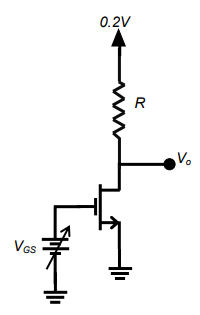
\includegraphics[width=0.25\linewidth]{exp2ckt}
	\caption{The circuit used in Experiment 2.}
	\label{fig:exp2ckt}
\end{figure}
\subsection{Procedure}
The follow steps were carried out, as instructed by the lab assignment.
\begin{enumerate}
	\item Using the same NMOS circuit, construct the circuit shown in Figure \ref{fig:exp2ckt}.
	\item Using the DC power supply, apply the calculated $V_{GS}$ values obtained earlier and use the DMM to measure the corresponding output voltage $V_o$. Calculate the error and record the data in the lab notebook.
	\item Vary $V_{GS}$ until the output voltage $V_o$ reaches the nominal values and record the error between the expected and measured gate voltage.
\end{enumerate}

\subsection{Results and analysis}
% state all measured values, graphs, tables, and figs.
% state any deviation from theoretical expected values
% use tables and graphs
% * must justify error in results otherwise the experiment failed
In this lab, we required a nominal resistance $R$ of \SI{42.84}{\ohm}. Using several resistors in series, the measured resistance was
\[ R = \SI{42.61}{\ohm} \quad (0.54\% \text{ error})\]
Using the $k_n$ value found in the last experiment and the gate voltages from the prelab, there was a high percent error, as shown in Table \ref{table:exp2values}. Our estimations for the gate voltages did not accurately reflect the measured output voltage, with an average error of 60\%. This high error is likely due to inaccuracies when measuring the $k_n$-value in the triode region. 
\begin{table}[H]
	\centering
	\caption{Measured output voltages using ideal input gate voltages.}
	\label{table:exp2values}
	\begin{threeparttable}
		\begin{tabular}{cccc}
			\toprule
			$V_{GS}$& Expected $V_o$ & Measured $V_o$ & \% error \\
			\midrule
			\SI{3.50}{\V} & \SI{0.02}{\V} & \SI{0.0141}{\V} & 29.5\% \\
			\SI{1.81}{\V} & \SI{0.1}{\V} & \SI{0.191}{\V} & 91.0\% \\
			\bottomrule
		\end{tabular}
	\end{threeparttable}
\end{table}
Next, we varied the gate voltage until the measured output voltage reached \SI{0.1}{\V} and \SI{0.02}{\V}. The gate voltages are shown in Table \ref{table:exp2varied}. During this part of the experiment, it was noted that minor changes in the gate voltage significantly impacted the measured output voltage. The transistor was very sensitive to changes across the gate and source. Here, we measured the error between the expected gate voltage and measured gate voltage. Again, the high error is likely due to a high error from Experiment 1 when determining the $k_n$ value for this transistor in the triode region.
\begin{table}[H]
	\centering
	\caption{Measured output voltage with the gate voltage varied.}
	\label{table:exp2varied}
	\begin{threeparttable}
		\begin{tabular}{cccc}
			\toprule
			$V_{GS}$& Expected $V_o$ & Measured $V_o$ & \% error \\
			\midrule
			\SI{2.62}{\V} & \SI{0.02}{\V} & \SI{0.01996}{\V} & 25.1\% \\
			\SI{2.00}{\V} & \SI{0.1}{\V} & \SI{0.10310}{\V} & 10.5\% \\
			\bottomrule
		\end{tabular}
	\end{threeparttable}
\end{table}

\subsection{Conclusion}
%  conclusion of the exp
This experiment utilized the NMOS transistor as a voltage-controlled resistor. While our expected voltages were roughly in the same order as the measured values, there was some significant deviation. This error was likely due to the imprecision when initially determining the $k_n$ values in Experiment 1, as noted earlier. Despite this, when we found the \textit{correct} values, the difference between the expected and measured gate voltage was only roughly 10--30\% off. Even if the $k_n$ were precisely accounted for, even a small difference in gate voltage would lead to significantly different output voltages, as noted by the difference in error between both parts of the experiment.

\pagebreak
%%%%%%%%%%%%%%%%%%%%%%%%%%%%%%%%%%%%%%%%%%%%%%%%%%%%%%%%%%%%%
\section{MOSFET as a buffer amplifier}

\subsection{Purpose}
% purpose of the experiment and its specs and/or design requirements
In this experiment, we explore using a MOSFET as a buffer amplifier. This amplifier is used to isolate an input signal source, which is unable to supply a load with a large current. With a MOSFET, the input signal can use the transistor as a buffer, allowing the transistor to drive the output load with a voltage proportional to the input.

\subsection{Theoretical background}
% background and its theory of operation, circuit diagrams, the main equations, results from the prelab
Shown in Figure \ref{fig:exp3ckt}, we will build a buffer amplifier, which will be used to drive a load with an equivalent voltage as the input $V_I$. We will use the IRF510 NMOS power transistor, in a TO220 package, and drive a decade box load with \SI{50}{\ohm} of resistance. If we determine the power utilized by the source, we can see that the power is minuscule, relative to the load power. This is shown below in Table \ref{table:exp3power}. This is due to the input current only being drawn by the resistor $R_G$ and only minimal (zero) current going into the transistor itself.
\begin{table}[H]
	\centering
	\caption{Power supplied by the source and power supplies at three input voltages.}
	\label{table:exp3power}
	\begin{threeparttable}
		\begin{tabular}{ccc}
			\toprule
			Input $V_{I}$ (V) & Input $P_{I}$ (W) & Power Supply $P_{dd}$ (W) \\
			\midrule
			$0$ & $0$ & $0$ \\
			$15$ & $0.10$ & $4.5$ \\
			$25$ & $0.28$ & $12.5$ \\
			\bottomrule
		\end{tabular}
	\end{threeparttable}
\end{table}
\begin{figure}[h]
	\centering
	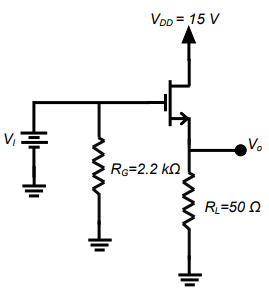
\includegraphics[width=0.3\linewidth]{exp3ckt}
	\caption{The buffer amplifier circuit, utilized in Experiment 3. Note: $V_{DD}$ is set to 15 volts in this figure, however, it was changed to 25 volts on the day of the experiment.}
	\label{fig:exp3ckt}
\end{figure}


\subsection{Procedure}
The follow steps were carried out, as instructed by the lab assignment.
\begin{enumerate}
	\item Construct the circuit shown in Figure \ref{fig:exp3ckt} using an IRF510 NMOS transistor. Use a decade box as the load resistor, set to 50 ohm. Measure and record the resistor values using the DMM. Use a DC power supply to supply $V_{DD} = 15$ V and the other amplifier at the gate of the transistor.
	\item Use DMM1 and DMM2 to measure the input and output voltage simultaneously. Determine the threshold voltage by starting $V_I$ at zero and slowly increasing the voltage until $V_O$ departs from zero. Record this voltage.
	\item In increments of a volt, we increased the gate voltage to 25 V and recorded this data in a table and calculate the power supplied by the input, and determine the regions.
	\item Using Excel, this data was recorded and plotted.
\end{enumerate}

\subsection{Results and analysis}
% state all measured values, graphs, tables, and figs.
% state any deviation from theoretical expected values
% use tables and graphs
% * must justify error in results otherwise the experiment failed
Using the DMM, the resistor voltages were measured as, \begin{align*}
	R_G & = \SI{2.1941}{\kohm} & (\SI{2.2}{\kohm}\text{ nominal, 0.3\% error}) \\
	R_{L} & = \SI{50.26}{\ohm} & (\SI{50}{\ohm}\text{ nominal, 0.5\% error})
\end{align*}
Next, the threshold voltage was found to be roughly \SI{2.25}{\V}, \begin{align*}
	V_I = \SI{2.25}{\V} & \to V_O = \SI{1e-6}{\V} \\
	V_I = \SI{2.5}{\V} & \to V_O = \SI{9e-6}{\V}
\end{align*}
In increments of a volt, we measured the corresponding output voltages and determined the regions using the NMOS equations from Table \ref{table:exp1current}. This data was collected in Excel (shown in the Appendix), then plotted in Figure \ref{fig:exp3regions}. The power supplied by the input was calculated, as well as the power delivered to the load, then plotted in Figure \ref{fig:exp3power}. Note that the power delivered to the load is not supplied by the input source, but rather is supplied by the power supply $V_{DD}$. Ideally, zero current (and power) from the source is delivered across the gate of the transistor.
\begin{figure}[H]
	\centering
	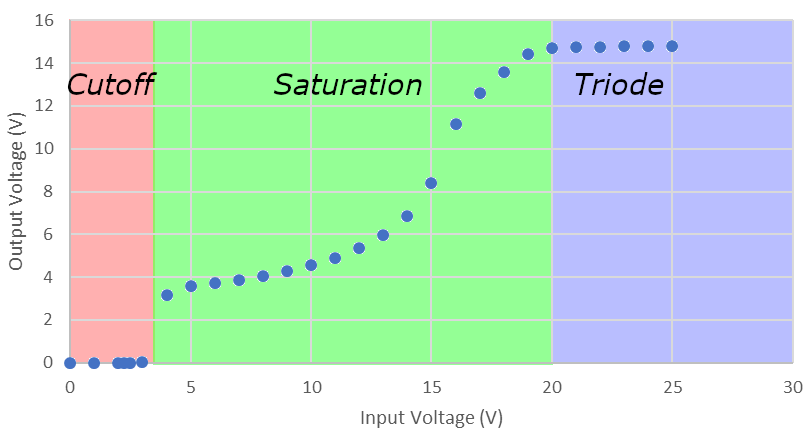
\includegraphics[width=0.7\linewidth]{exp3regions}
	\caption{The input/output voltages of the buffer amplifier and their corresponding regions.}
	\label{fig:exp3regions}
\end{figure}
\vspace{-2em}
\begin{figure}[H]
	\centering
	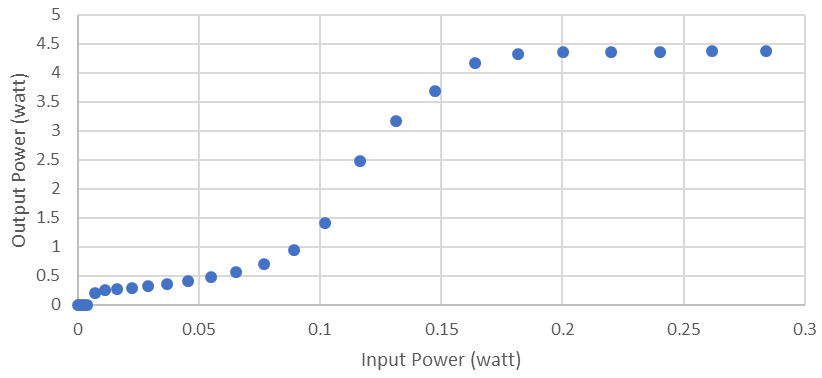
\includegraphics[width=0.7\linewidth]{exp3power}
	\caption{The input power vs the output power.}
	\label{fig:exp3power}
\end{figure}
\vspace{-2.5em}
\subsection{Conclusion}
In this last experiment, we used the NMOS transistor as a buffer amplifier, allowing an low-current input to drive a high-current output. This application takes advantage of the zero-input-current characteristics of the transistor gate. Rather, the power supplied to the load is coming from the power supply at $V_{DD}$. In this part, the transistor is operated under each: the cut-off region, saturation, then lastly, the triode region. The transistor behaves differently in each region, where the transistor is off until the threshold current is reached.
\pagebreak
\section*{Appendix}
\begin{table}[H]
	\caption{Data collected during Experiment 3.}
	\centering
	\begin{tabular}{@{}lllll@{}}
		\toprule
		$V_i$ (V) & $V_o$ (V) & Region            & $P_i$ (W)    & $P_o$ (W) \\ \midrule
		0        & 0        & cutoff            & 0           & 0.00     \\
		1        & 0        & cutoff            & 0.000454545 & 0.00     \\
		2        & 0        & cutoff            & 0.001818182 & 0.00     \\
		2.25     & 0.00001  & cutoff            & 0.002301136 & 0.00     \\
		2.5      & 0.00009  & cutoff/saturation & 0.002840909 & 0.00     \\
		3        & 0.01187  & cutoff/saturation & 0.004090909 & 0.00     \\
		4        & 3.17     & saturation        & 0.007272727 & 0.20     \\
		5        & 3.57     & saturation        & 0.011363636 & 0.25     \\
		6        & 3.70     & saturation        & 0.016363636 & 0.27     \\
		7        & 3.86     & saturation        & 0.022272727 & 0.30     \\
		8        & 4.05     & saturation        & 0.029090909 & 0.33     \\
		9        & 4.28     & saturation        & 0.036818182 & 0.37     \\
		10       & 4.56     & saturation        & 0.045454545 & 0.42     \\
		11       & 4.90     & saturation        & 0.055       & 0.48     \\
		12       & 5.35     & saturation        & 0.065454545 & 0.57     \\
		13       & 5.96     & saturation        & 0.076818182 & 0.71     \\
		14       & 6.87     & saturation        & 0.089090909 & 0.94     \\
		15       & 8.42     & saturation        & 0.102272727 & 1.42     \\
		16       & 11.14    & saturation        & 0.116363636 & 2.48     \\
		17       & 12.60    & saturation        & 0.131363636 & 3.17     \\
		18       & 13.57    & saturation        & 0.147272727 & 3.68     \\
		19       & 14.43    & saturation        & 0.164090909 & 4.16     \\
		20       & 14.71    & triode            & 0.181818182 & 4.33     \\
		21       & 14.75    & triode            & 0.200454545 & 4.35     \\
		22       & 14.77    & triode            & 0.22        & 4.36     \\
		23       & 14.78    & triode            & 0.240454545 & 4.37     \\
		24       & 14.79    & triode            & 0.261818182 & 4.37     \\
		25       & 14.79    & triode            & 0.284090909 & 4.37     \\ \bottomrule
	\end{tabular}
\end{table}
\end{document}